\section{BlueJ}
\label{sec:bluej}

\todo{Results and discussion.}

\subsection{Fibonacci}
The Fibonacci sequence in BlueJ can be expressed both by using an iterative and recursive approaches. An example could be seen in \figref{fig:bluej_fibo_code2}, where the user is prompted to give a number and the respective result is shown.

\begin{figure}[!h]
  \centering
    \begin{subfigure}[b]{0.45\textwidth}
    \begin{center}
      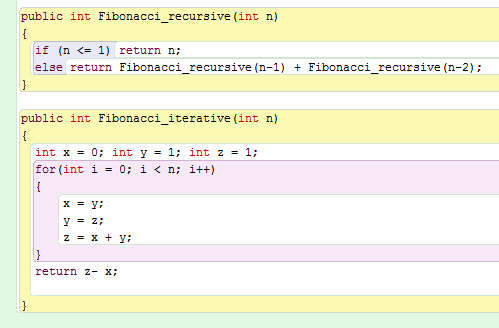
\includegraphics[scale=0.7]{./pics/bluej_fibo_code}
      \caption{BlueJ Fibonacci code.}
      \label{fig:bluej_fibo_code}
    \end{center}
    \end{subfigure}
    ~
    \begin{subfigure}[b]{0.45\textwidth}
    \begin{center}
      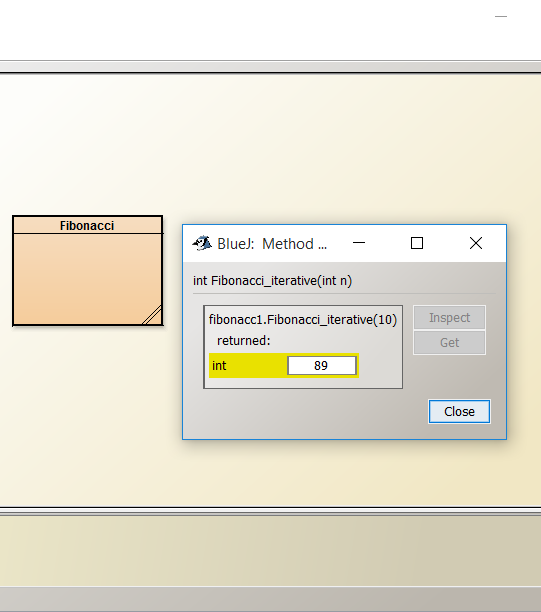
\includegraphics[scale=0.6]{./pics/bluej_fibo_code2}
      \caption{BlueJ Fibonacci output.}
      \label{fig:bluej_fibo_code2}
    \end{center}
    \end{subfigure}
    \caption{Code and output for Fibonacci numbers.}
    \label{fig:bluej_fibo}
\end{figure}
\subsection{Cups and Ball}
Similarly to how this game was implemented in Scratch, it gives the player the chance to guess where a ball might be among 15 identical cups, but it feels less intuitive since there is no visual feedback given but rather textual one - that the player has either successfully guessed the position of the ball or not. The example can be seen in \figref{fig:bluej_ballcup_code} 

\begin{figure}[!h]
  \centering
      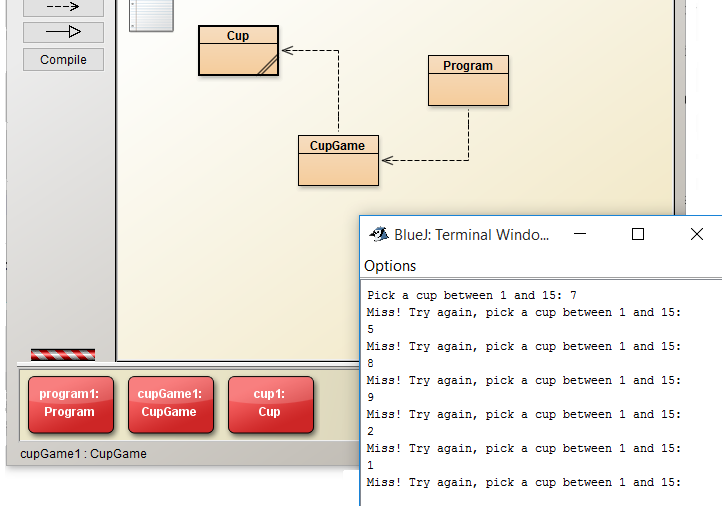
\includegraphics[scale=0.7]{./pics/bluej_ballcup_code}
      \caption{Code and output for Cups and Ball..}
      \label{fig:bluej_ballcup_code} 
\end{figure}

\subsection{Hangman}
The Hangman is also a guessing game where the player has to guess a particular word by providing one letter at the time. If the letter is part of the word, the its added to a guessing list, otherwise if it not, it is added to the wrong list instead. Every time the player gives a wrong letter, one of his lifes is long, and thus he loses the game if he loses all of them. Since BlueJ uses Java as the underlying language, the code follows an imperative style of programming with conditional statements and loops, some of which are illustrated on \figref{fig:bluej_hangman_code} 

\begin{figure}[!h]
  \centering
      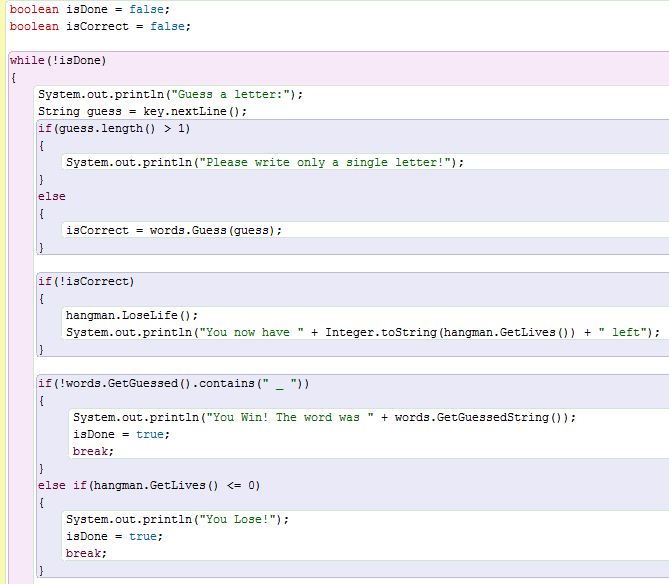
\includegraphics[scale=0.7]{./pics/bluej_hangman_code}
      \caption{Code for Hangman game}
      \label{fig:bluej_hangman_code} 
\end{figure}
\subsection{Iterator}

\subsection{Criteria Evaluation}
\begin{description}[style=nextline]
\item[Readability]
\item[Writability]
\item[Observability]
\item[Trialability]
\item[Learnability]
\item[Reusability]
\item[Pedagogic Value]
\item[Environment]
\item[Documentation]
\end{description}